\chapter{Theoretical Foundations}\label{ch:theory}

This chapter explains the theory behind the final ECG system. It follows the
actual implementation: a one-lead MLII beat classifier that uses waveform
shape, RR timing, autoencoder residuals, and two supervised Extra Trees
ensembles. The chapter does not assume a second ECG lead or an offline
record-summary input, because the deployed model does not use those inputs.

\section{Why ECG evidence has more than one form}

An ECG is a voltage signal over time. For arrhythmia classification, useful
evidence appears at two related scales. The first is beat-scale morphology:
what the P--QRS--T shape looks like around one R peak. The second is rhythm
timing: when the beat occurs relative to neighbouring beats. The final model
uses both because they answer different questions.

\begin{figure}[H]
\centering
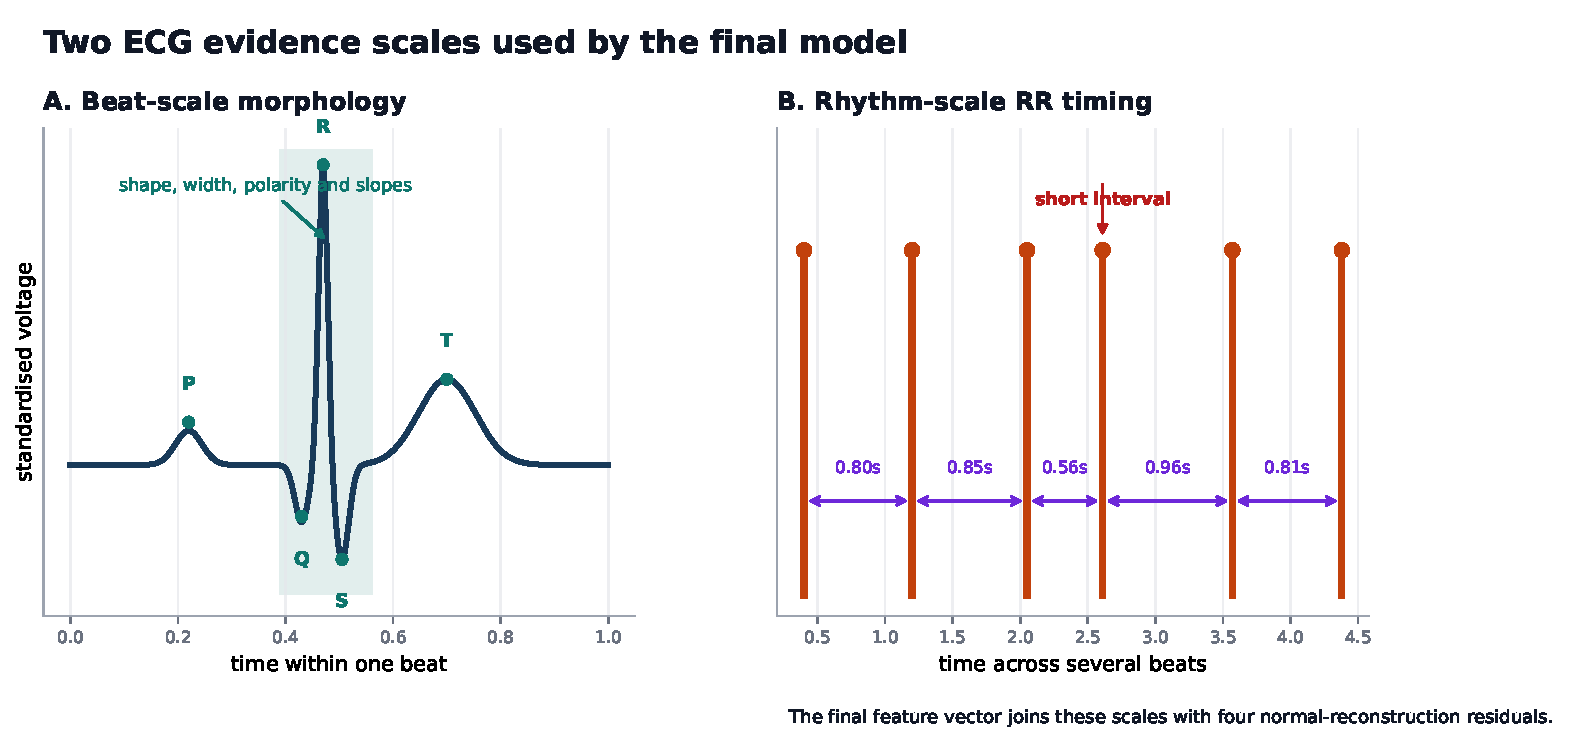
\includegraphics[width=.98\textwidth]{pic/generated/theory_evidence_scales.pdf}
\caption{Two evidence scales used by the final model. Morphology describes the
local shape of a beat; RR timing describes rhythm context around the beat.}
\label{fig:theory-evidence-scales}
\end{figure}

PVC, LBBB, and RBBB can strongly affect QRS shape, width, slopes, and polarity.
PAC and AFib may be easier to detect when timing evidence is also present:
premature beats create short RR intervals, pauses create long RR intervals, and
AFib creates repeated irregularity. Published heartbeat-classification work
also shows the value of combining waveform morphology with heartbeat-interval
features \cite{dechazal2004heartbeat,mousavi2019seq2seq}.

\section{Feature extraction theory}

The raw 512-sample MLII window contains more detail than the final tree models
need. Small changes in R-peak alignment or noise can change many raw sample
values. The system therefore converts the window into compact measurements
that keep useful ECG evidence while reducing unnecessary sample-level detail.

\begin{figure}[H]
\centering
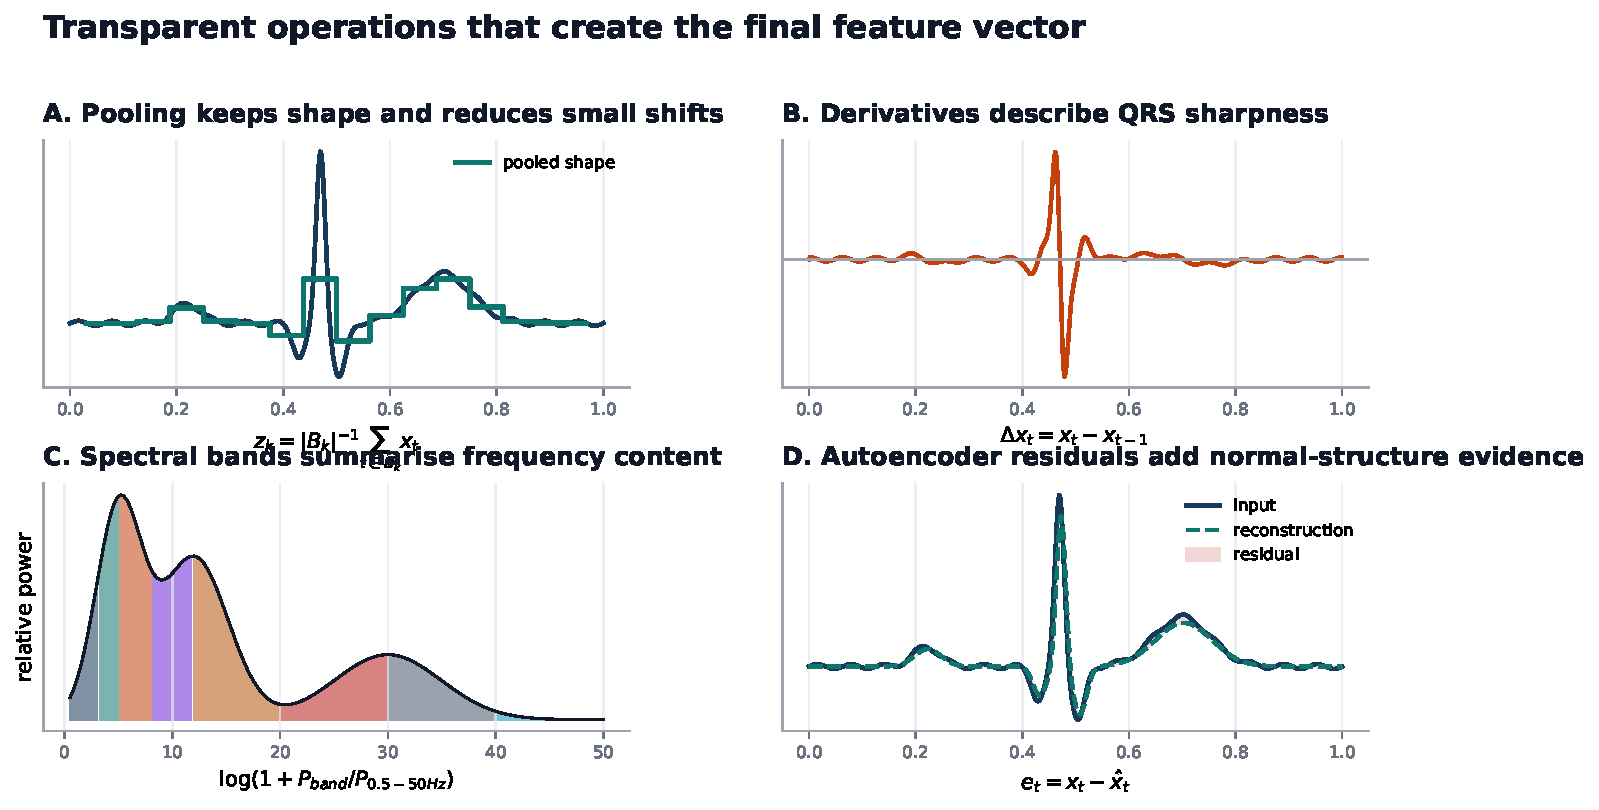
\includegraphics[width=.98\textwidth]{pic/generated/theory_feature_math.pdf}
\caption{Feature-extraction operations behind the final 242-value vector. The
tree models learn from compact numerical evidence, not from raw ECG samples
directly.}
\label{fig:theory-feature-math}
\end{figure}

For a pooled region $B_k$, the pooled value is
\begin{equation}
 z_k=\frac{1}{|B_k|}\sum_{t\in B_k}x_t.
\end{equation}
Pooling keeps the average shape in a small region and makes the representation
less sensitive to a one- or two-sample shift. The final system uses 64
whole-window pooled values and 80 central morphology pooled values.

The derivative
\begin{equation}
 \Delta x_t=x_t-x_{t-1}
\end{equation}
describes how quickly voltage changes. This matters because QRS abnormalities
often change slopes and sharpness. The system keeps 60 pooled derivative values
from the central beat region.

Frequency features describe how signal energy is spread from 0.5 to 50~Hz. For
a frequency band $b$, the relative band feature is
\begin{equation}
 s_b=\log\left(1+\frac{P_b}{P_{0.5-50}}\right),
\end{equation}
where $P_b$ is the power inside the band and $P_{0.5-50}$ is total power in the
ECG band used by the feature extractor. This band-limited view follows the
general ECG idea of keeping physiological content while reducing drift and
high-frequency interference
\cite{kligfield2007standardization,butterworth1930filter}.

Eleven summary statistics add scale, range, energy, skewness, and kurtosis.
Together, the waveform, derivative, spectral, and statistical values form 223
non-RR, non-autoencoder features.

\section{RR timing theory}

Let $r_i$ be the time of the R peak of beat $i$. The RR interval is
\begin{equation}
 RR_i=r_i-r_{i-1}.
\end{equation}
RR values describe rhythm. A short interval can suggest a premature beat. A
long interval can suggest a pause. Repeated interval changes support rhythm
irregularity.

The final live system classifies a beat only after it has enough context to
compute the same RR information used in the final experiment. It uses seven
base RR values, including previous RR, next RR, local mean RR, interval ratios,
local coefficient of variation, and heart rate. It then appends eight
history-based values from already completed intervals: median, interquartile
range, median absolute deviation, RMSSD, pNN50, relative range, trend, and
latest interval change.

RMSSD is one example:
\begin{equation}
 \mathrm{RMSSD}=\sqrt{\frac{1}{K-1}\sum_{j=2}^{K}(RR_j-RR_{j-1})^2}.
\end{equation}
The next-RR requirement is important. It creates a small beat-level delay during
streaming, but it also makes the live RR feature vector match the experiment.

\section{Normal-only reconstruction theory}

An autoencoder contains an encoder $f_\theta$ and decoder $g_\phi$. It is
trained to reconstruct a normal ECG window $x$:
\begin{equation}
 \hat{x}=g_\phi(f_\theta(x)), \qquad
 \min_{\theta,\phi}\frac{1}{T}\sum_{t=1}^{T}(x_t-\hat{x}_t)^2.
 \label{eq:ae-objective}
\end{equation}
This follows the representation-learning idea of autoencoders
\cite{hinton2006autoencoder}. The final autoencoder is trained with a
denoising objective: small Gaussian noise is added to the input while the
target remains the clean normal window. Denoising encourages stable structure
instead of exact noise copying \cite{vincent2008denoising}.

\begin{figure}[H]
\centering
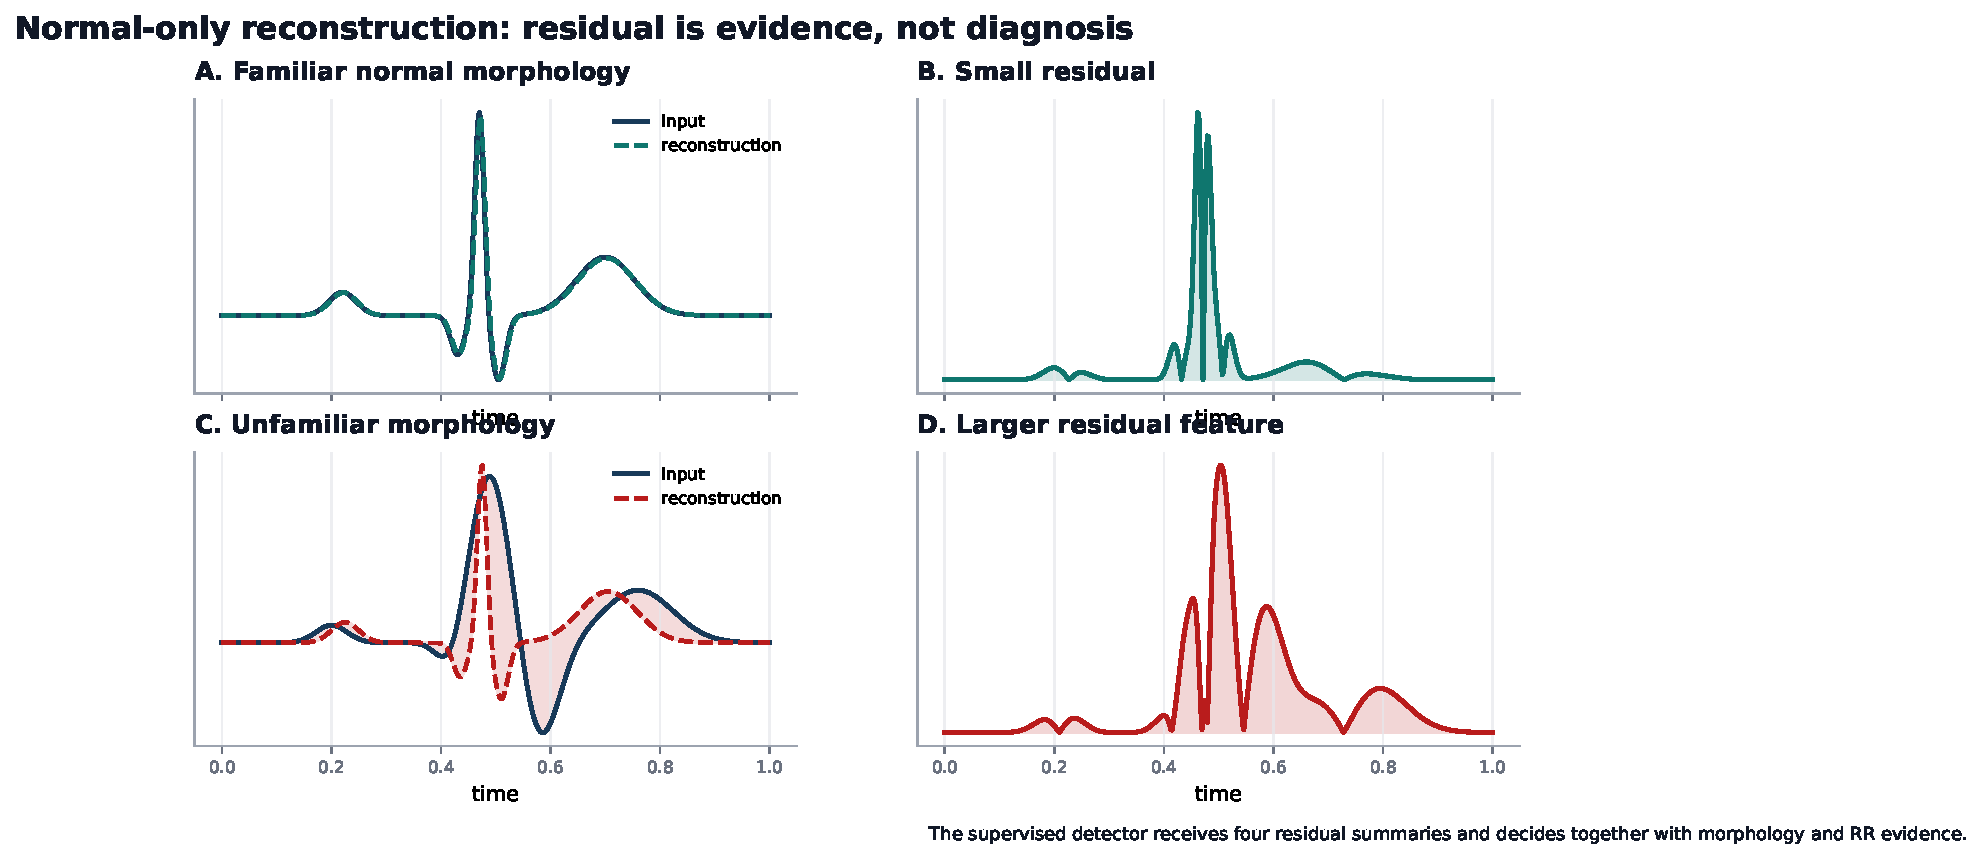
\includegraphics[width=.98\textwidth]{pic/generated/theory_reconstruction_principle.pdf}
\caption{Normal-only reconstruction principle. A larger residual can indicate
novelty, but it is evidence only; the final arrhythmia decision is made by the
supervised hierarchy.}
\label{fig:theory-reconstruction-principle}
\end{figure}

If the autoencoder has learned common normal structure, an unfamiliar or
abnormal beat may be reconstructed less accurately. This is the one-class
anomaly detection idea \cite{chandola2009anomaly}. It is not a guarantee. A
flexible decoder may reconstruct an abnormal waveform well, and noise may
create a large residual for a normal waveform. Therefore, the final system uses
autoencoder mismatch as four supervised input features, not as the final
diagnosis rule.

Let $e_t=x_t-\hat{x}_t$ be the residual. The four residual features are:
\begin{align}
 e_{\mathrm{MAE}} &= \frac{1}{T}\sum_t |e_t|,\\
 e_{\mathrm{MSE}} &= \frac{1}{T}\sum_t e_t^2,\\
 e_{\mathrm{local}} &= \frac{1}{|Q|}\sum_{t\in Q}|e_t|,\\
 e_{\Delta} &= \frac{1}{T-1}\sum_{t=2}^{T}|e_t-e_{t-1}|.
\end{align}
They measure whole-window mismatch, squared mismatch, central morphology
mismatch, and residual sharpness. The final architecture appends these four
values to the MLII waveform and RR features.

\section{Hierarchical classification theory}

The final problem is not solved with one direct classifier. The system first
asks whether the beat is abnormal. Only when this binary gate is true does it
ask which supported abnormal subtype is most likely.

\begin{figure}[H]
\centering
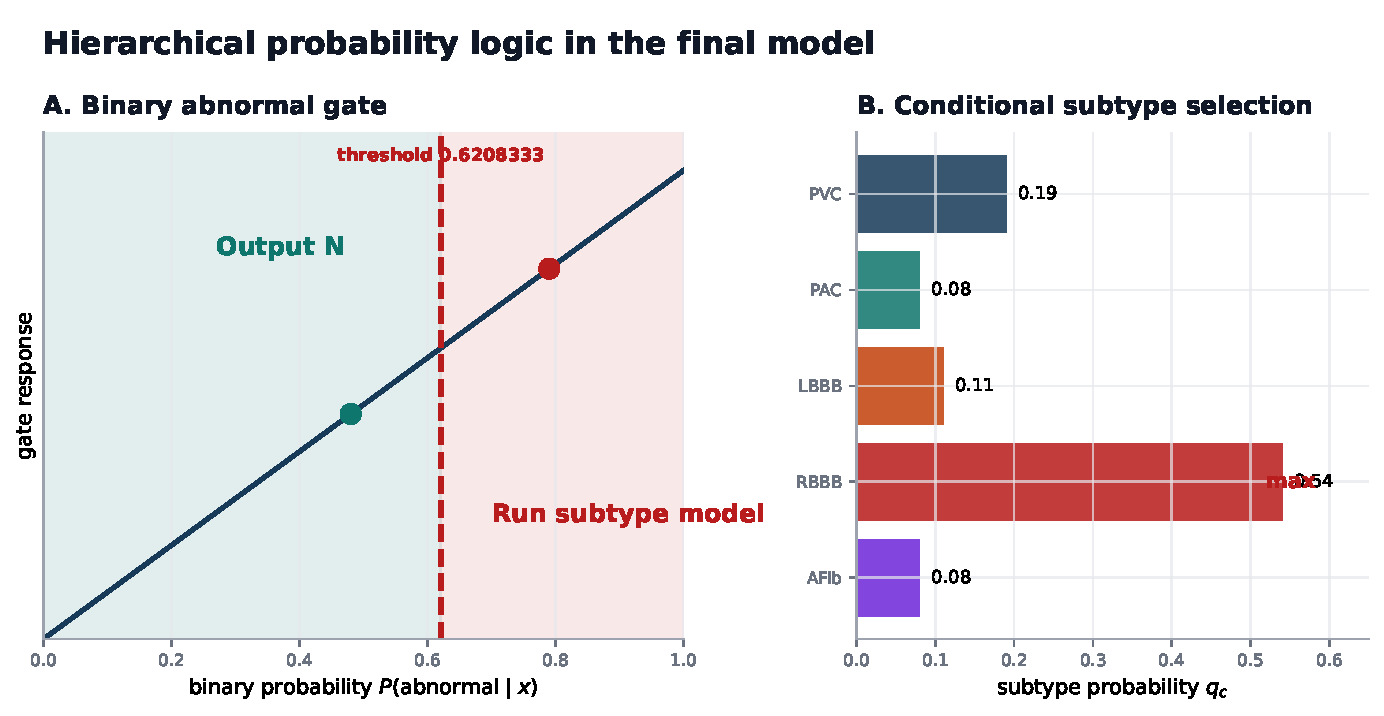
\includegraphics[width=.98\textwidth]{pic/generated/theory_hierarchy_probability.pdf}
\caption{Probability logic of the final hierarchy. The subtype model is
conditional: it is used only after the abnormality gate is passed.}
\label{fig:theory-hierarchy-probability}
\end{figure}

For beat $i$, the binary detector estimates $p_i=P(\mathrm{abnormal}\mid x_i)$.
The final threshold rule is
\begin{equation}
 a_i=\mathbb{1}[p_i>0.6208333].
\end{equation}
If $a_i=0$, the output is N. If $a_i=1$, the subtype model selects the highest
probability among PVC, PAC, LBBB, RBBB, and AFib:
\begin{equation}
 \widehat y_i=1+\arg\max_{c\in\{1,\ldots,5\}}q_{ic}.
\end{equation}
This hierarchy has a practical advantage. Unsupported abnormal MIT--BIH symbols
can still contribute to binary abnormality testing without being forced into
one of the five supported subtype labels.

\section{Why Extra Trees fits this feature design}

The final 242-value vector mixes pooled waveform values, derivatives, spectral
power, signal statistics, RR timing, and autoencoder residuals. Their
relationship to class labels is non-linear. Extra Trees fits this setting by
building many randomised decision trees and averaging their probability
outputs.

At a decision-tree node with class probabilities $p_c$, entropy is
\begin{equation}
 H=-\sum_c p_c\log_2 p_c.
\end{equation}
A split is useful when it reduces the weighted child entropy. Extra Trees adds
randomness by selecting random feature subsets and random split candidates.
Averaging many such trees reduces the instability of a single tree while
retaining non-linear interactions between features.

This theory also explains why Extra Trees is suitable for the final data scale.
MITDB contributes many beats but only 45 subject clusters. A very high-capacity
end-to-end neural classifier could learn patient identity instead of robust ECG
rules \cite{zhang2021interpatient}. The Extra Trees hierarchy is still
high-capacity, but it uses transparent tabular evidence and is easier to audit
against the final temporal protocol. This does not mean that tree ensembles are
always better than deep learning.

\section{Class and patient imbalance theory}

ECG beat datasets are imbalanced in two ways. Some classes are rare, and some
patients contribute many more beats than others. Without weighting, a model can
mostly learn common normal beats or a few large records.

The final training code uses record-aware class weights. For class $c$ in
record $r$, the weight is proportional to
\begin{equation}
 w_{cr}=\frac{1}{n_c}
 \left(\frac{n_c}{R_c n_{cr}}\right)^\alpha,
 \label{eq:record-weight}
\end{equation}
where $n_c$ is total support for class $c$, $R_c$ is the number of records
containing class $c$, and $n_{cr}$ is the number of class-$c$ beats in record
$r$. The first factor supports class balancing; the second factor reduces
domination by a single record. The exponent $\alpha$ controls how strongly
record balancing is applied and is selected in validation. Class-balanced
learning is important when rare classes would otherwise have little influence
\cite{cui2019classbalanced}.

\section{Temporal patient adaptation theory}

ECG morphology contains patient-specific information such as body geometry,
electrode placement, baseline QRS shape, conduction pattern, and background
rhythm. If earlier labelled ECG from a patient is available during development,
the model can adapt to that patient's baseline. Later ECG from the same patient
is then easier than ECG from a completely unseen patient.

This is the theory behind the final temporal-holdout design. It is useful for
monitoring after a labelled calibration period, but it changes the claim. The
final result is a known-patient temporal-continuation result. It should not be
reported as unseen-patient generalisation unless a patient-disjoint experiment
is run. The 16-beat boundary gap reduces direct overlap at the split boundary,
but it does not remove shared patient identity.

\section{Validation theory}

Beat-level accuracy alone is not enough. If one patient contributes 2,000
beats, those beats are related. They are not equivalent to 2,000 independent
patients. The final validation therefore reports beat metrics and also uses
subject-clustered uncertainty.

\begin{figure}[H]
\centering
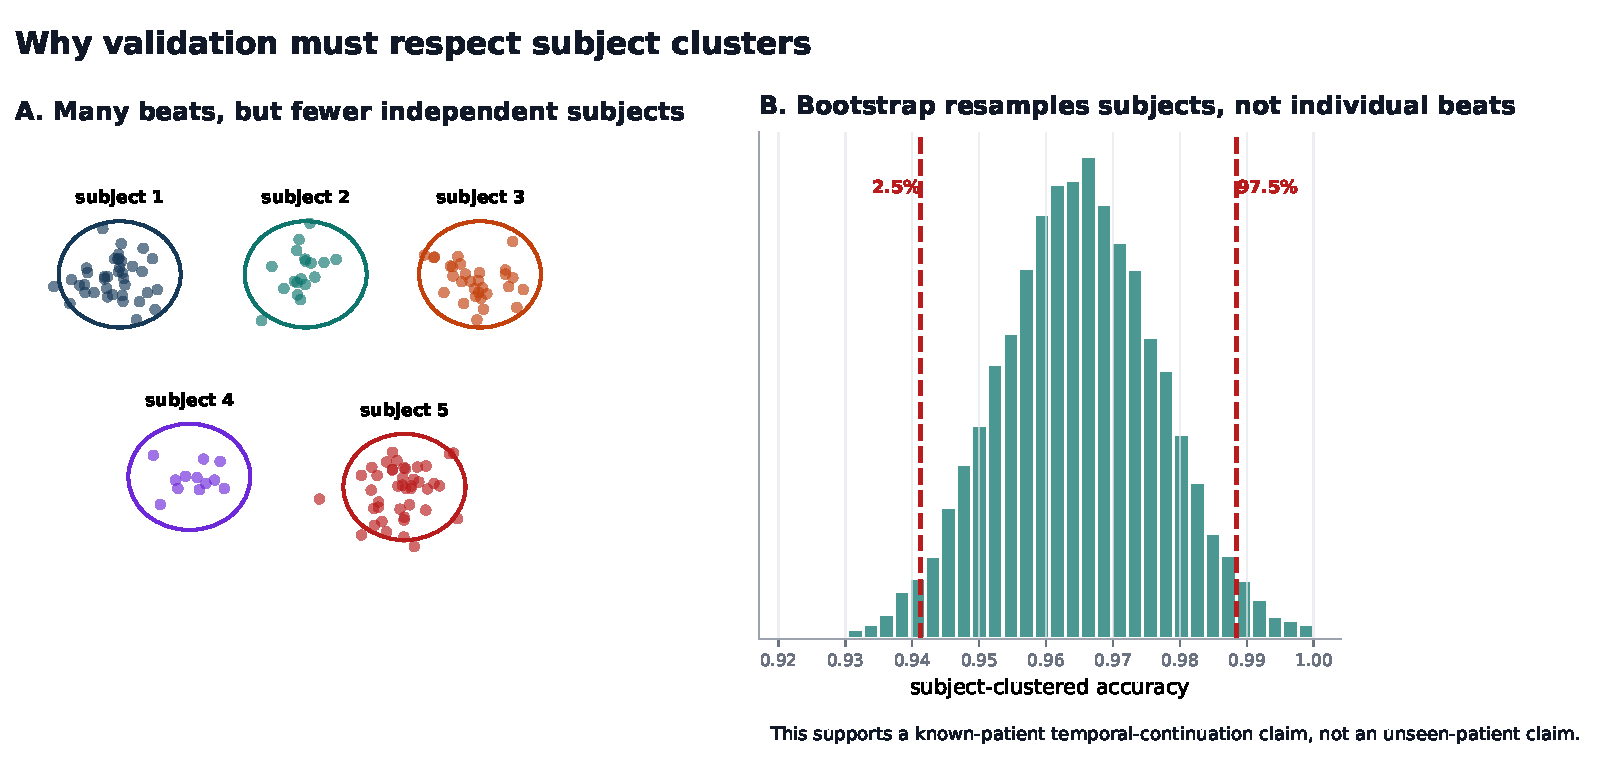
\includegraphics[width=.98\textwidth]{pic/generated/theory_validation_units.pdf}
\caption{Theoretical reason for subject-clustered validation. Clustered
resampling prevents one long record from being treated as many independent
people.}
\label{fig:theory-validation-units}
\end{figure}

Balanced accuracy gives equal weight to class recalls, so normal beats cannot
hide poor abnormal recall. Macro F1 gives each class equal importance, so a
failure on a rare class is visible. Precision--recall style measures are also
important under class imbalance \cite{saito2015pr}. For confidence intervals,
the final experiment resamples complete subject clusters rather than individual
beats, following the general diagnostic-statistics principle that clustered
data need clustered analysis \cite{rutter2000clustered}.

\section{Theory-to-system alignment}

\begin{table}[H]
\centering
\caption{How the theory maps to the implemented final system.}
\label{tab:theory-system-alignment}
\begin{tabular}{>{\raggedright\arraybackslash}p{4.2cm}>{\raggedright\arraybackslash}p{9.0cm}}
\toprule
Theory concept & Implemented in the final system\\
\midrule
Beat-scale morphology & 512-sample MLII window with pooled full-window,
central, and derivative features\\
Rhythm timing & 15 RR features; live scoring waits until next-RR context is
available\\
Normal-only reconstruction & frozen NSRDB autoencoder supplies four residual
features\\
Hierarchical probability & 240-tree binary gate first; 260-tree subtype model
only for gated abnormal beats\\
Class/patient imbalance & record-aware class weighting with validation-selected
record-power parameter\\
Temporal adaptation & earlier MLII timeline trains/selects the model; final
20\% timeline is tested\\
Subject-aware uncertainty & subject-clustered bootstrap over 45 clusters, with
records 201 and 202 treated as one cluster\\
\bottomrule
\end{tabular}
\end{table}
